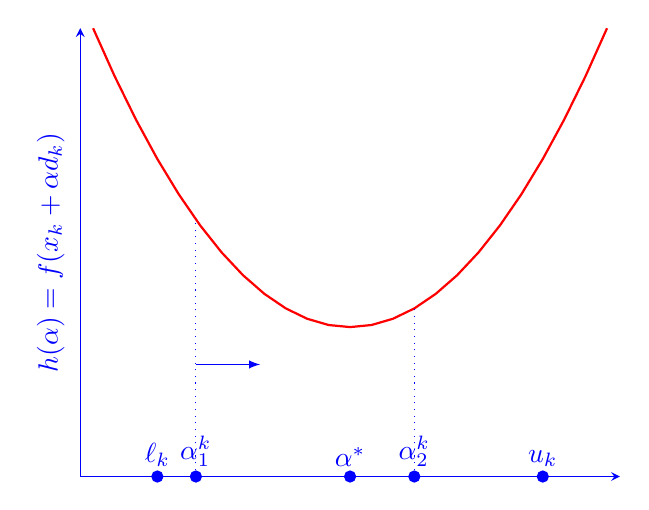
\begin{tikzpicture}[blue]
  \begin{axis}[
      domain=-2:2,
      axis lines=left,
      xtick=\empty,
      ytick=\empty,
      xmin=-2.1,
      xmax=2.1,
      ylabel={$h(\alpha)= f(x_k + \alpha d_k)$},
    ]
    \addplot[thick, red, mark=none] {x*x+1)};
    \addplot[mark=*] coordinates { (-1.5, -1) };
    \node[anchor = south] at (axis cs: -1.5, -1) {$\ell_k$};
    \addplot[mark=*] coordinates { (1.5, -1) };
    \node[anchor = south] at (axis cs: 1.5, -1) {$u_k$};
    \addplot[mark=*] coordinates { (-1.2, -1) };
    \addplot[mark=none, dotted] coordinates { (-1.2, -1) (-1.2, 1+1.2*1.2) };
    \node[anchor = south] at (axis cs: -1.2, -1) {$\alpha^k_1$};
    \addplot[mark=*] coordinates { (0, -1) };
    \node[anchor = south] at (axis cs: 0, -1) {$\alpha^*$};
    \addplot[mark=*] coordinates { (0.5, -1) };
    \addplot[mark=none, dotted] coordinates { (0.5, -1) (0.5, 1+0.5*0.5) };
    \node[anchor = south] at (axis cs: 0.5, -1) {$\alpha^k_2$};
    \draw[-latex](axis cs:-1.2, 0.5)--(-0.7, 0.5);
  \end{axis}
\end{tikzpicture}
